% !TEX root = ../../book.tex
\chapter{Dynamic Portfolio Management and Trading Strategies \label{ch:amp}}
\section{Introduction to Modern Portfolio Theory \label{s:mod_port_theory}}

Of fundamental interest to financial economists is to examine the relationship between the risk of a financial security and its return. While it is obvious that risky assets can generally yield higher returns than risk-free assets, a quantification of the tradeoff between risk and expected return was made through the development of the Capital Asset Pricing Model (CAPM) for which the groundwork was laid by Markowitz (1959)~\cite{markport}. A central feature of the CAPM is that the expected return is a linear function of the risk. The risk of an asset typically is measured by the covariability between its return and that of an appropriately defined `market' portfolio. Models of expected return-risk relationships include the Sharpe (1964)~\cite{sharpcap} and Lintner (1965)~\cite{lint65} CAPM, the zero-beta CAPM of Black (1972)~\cite{blackcap}, the arbitrage pricing theory (APT) due to Ross (1976)~\cite{rossarb} and the intertemporal asset pricing model by Merton (1973)~\cite{mertonint}. The economy-wide models developed by Sharpe, Lintner and Black are based on the work of Markowitz which assumes that investors would hold a mean-variance efficient portfolio. The main difference between the work of Sharpe and Lintner and the work of Black is that the former assumes the existence of a risk-free lending and borrowing rate whereas the latter derived a more general version of the CAPM in the absence of a risk-free rate.


In this section, we briefly review the CAPM model and the implications for empirical research in the area of portfolio construction and testing. 



% Mean-Variance Portfolio Theory
\subsection{Mean-Variance Portfolio Theory}


A portfolio which is composed of individual assets has its risk and return characteristics based on its composition and how the individual asset characteristics correlate with each other. The optimal combination is designed to produce the best balance between risk and return. For a given level of return, it will provide the lowest risk and for an acceptable level of risk, it will provide the maximum return. The locus of the combination of risk and reward that characterizes the optimal portfolios is called the ``Efficient Frontier.''


We follow the same conventions as before to denote the return as $r_t= \ln(P_t) - \ln(P_{t-1})$; assume we have `$m$' assets in the portfolio with `$w_i$' denoting the share value invested in asset, `$i$', if $R_t=(P_t-P_{t-1})/P_{t-1}$, the portfolio return is $R_{pt}= \sum_{i=1}^m w_i R_{it}$ and thus $r_t= \ln \left(1+\sum_{i=1}^m w_i R_{it} \right) \simeq \sum_{i=1}^m w_i r_{it}$. If $r_t$ denotes the vector of `$m$' asset returns and with weights stacked up as a vector, $w$, then $r_{pt}= w' r_t$ resulting in $\mu_p= E(r_{pt})= w' \mu$ and $\sigma_p^2= w' \Sigma w$, where $\Sigma$ is the $m \times m$ variance-covariance matrix of $r_t$. If the returns are uncorrelated or negatively correlated, then observe that
	\begin{equation} \label{eqn:5sigmap}
	\sigma_p^2= w' \Sigma w \leq \sum_{i=1}^m w_i \Var(r_{it}) \leq \dfrac{v}{m},
	\end{equation}
where `$v$' is the maximum of $\var(r_{it})$, clearly indicating that diversification tends to reduce risk. The power of the diversification can be seen clearly if we assume the covariance matrix, $\Sigma$, has all variances equal and if all off-diagonal covariance elements are the same. Then, $\sigma_p^2= \frac{1}{n} \cdot \sigma^2 + \frac{n-1}{n} \cdot \rho \cdot \sigma^2$. Observe that if $\rho= 0$, $\sigma_p^2 \to 0$ as $n \to \infty$ and if $\rho= 1$, $\sigma_p^2= \sigma^2$ that results in no benefit. When $\rho < 0$ as shown in \eqref{eqn:5sigmap}, the portfolio variance is less due to diversification. But it should be noted that we cannot completely eliminate portfolio risk when the correlations among the assets are positive. Observe that $\sigma_p^2= \frac{1}{m^2} \sum_{i=1}^m \sigma_i^2 + \frac{1}{m^2} \sum_{i \neq j} \sigma_{ij} \leq \frac{\sigma_{\text{max}}^2}{m} + \frac{m-1}{m} \cdot A \to A$ as $m \to \infty$. Some amount of risk will remain if the portfolio consists of assets that move with the market. \\


\noindent\textbf{Minimum Variance Portfolio:} The efficient portfolio is obtained through the constrained optimization:
	\begin{equation} \label{eqn:5opt}
	\min_w w' \Sigma w \enskip \ni w' \mu = \mu^*, \quad w'1= 1.
	\end{equation}
Here 1 is the $m \times 1$ unit vector. The solution to this can be obtained via Lagrangian function and can be found in Campbell, Lo and MacKinley (1996)~\cite[Section 5.2]{campbellmaclo}. With $A= 1' \Sigma^{-1} \mu$ (weighted mean), $B= \mu' \Sigma^{-1} \mu$ ($F$-ratios), $C= 1' \Sigma^{-1}1$ and $D= BC - A^2$, the `weight' vector, $w$, is given as,
	\begin{flalign} \label{eqn:5effdoub}
	&& w_{\text{eff}}&= \{ B \Sigma^{-1} 1- A \Sigma^{-1}\mu + \mu^*(C\Sigma^{-1} \mu- A\Sigma^{-1}1)\}/D && \notag \\
	\text{and} && \phantom{x} & \phantom{x} && \\
	&& \sigma_{\text{eff}}^2&= (B - 2\mu^*A + \mu^{*2}C)/D. && \notag
	\end{flalign}
The graph of the efficient frontier $(\mu^*, \sigma_{\text{eff}})$ in the mean-standard deviation space is the right side of a hyperbola (see Figure~\ref{fig:frontier}).

	\begin{figure}[h!]
	   \centering
	   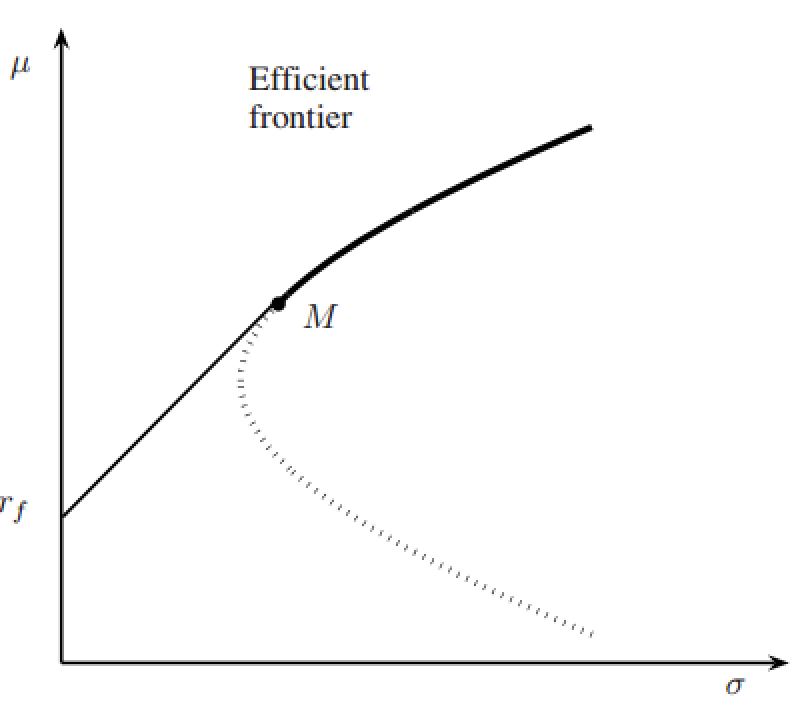
\includegraphics[width=0.6\textwidth]{chapters/chapter_apm/figures/frontier.png} 
	   \caption{Efficient frontier with no short selling. \label{fig:frontier}}
	\end{figure}
It must be noted that in the formulation \eqref{eqn:5opt}, the weights can be negative implying that short selling is allowed. With no short selling, $w_i \geq 0$ for all `$i$', there is no explicit solution but can be numerically solved via quadratic programming. 


Suppose an investor is interested in a portfolio with maximum Sharpe ratio ($=$ average return/standard deviation), which represents the return per unit risk. Graphically, the portfolio is the point where a line through the origin is tangent to the efficient frontier, because this point represents the highest possible Sharpe ratio. So it is called the tangency portfolio. The inverse of the slope is obtained by setting $\frac{\delta \sigma^2_{\text{eff}}}{\delta \mu^*}= 0$ which yields $\mu^*= A/C$ and $\sigma_{\text{MV}}^2= \frac{1}{C}$ and the efficient combination is simply, $w_{\text{MV}}= \Sigma^{-1} \mu/C$. Thus we have described two portfolios that an investor can prefer. If minimum amount of risk is desired, the minimum variance portfolio is taken and if the objective is to maximize the Sharp ratio, the tangency portfolio is taken. These can be formulated from the point of view of unified theory of utility maximization. 


Assume that the utility function is given as,
	\begin{equation} \label{eqn:utility}
	u= w' \mu - \frac{\lambda}{2} \,w' \,\Sigma \,w,
	\end{equation}
where `$\lambda$' is called the parameter of absolute risk-aversion. The greater the `$\lambda$', the more risk averse the investor is. Usually $2<\lambda<4$. Thus assuming all investors are risk-averse, the objective function is,
	\begin{equation} \label{eqn:5maxu}
	\max_w u \enskip \ni \enskip w'1= 1.
	\end{equation}
It can be easily shown that the resulting weight vector is,
	\begin{equation}\label{eqn:5weff}
	w_{\text{eff}}= \dfrac{1}{\lambda} \left(\Sigma^{-1} \mu + \Sigma^{-1} 1 \cdot \gamma^*\right),
	\end{equation}
where $\gamma^*= (\lambda - A)/C$. The results can be obtained again using Lagrangian multipliers and the matrix differentiation results $\left( \frac{\delta \Sigma w}{\delta w}= \Sigma; \frac{\delta(w' \Sigma w)}{\delta w})= 2 \cdot w' \Sigma \right)$. From \eqref{eqn:5weff}, observe that it is a combination of minimum variance portfolio and the tangency portfolio. At the optimum point, note
	\begin{flalign} \label{eqn:5effdoub1}
	&& \mu_{\text{opt}}&= w' \mu= \dfrac{D}{\lambda C}+\mu_{\text{MV}} && \notag \\
	\text{and} && \phantom{x} & \phantom{x} && \\
	&& \sigma^2_{\text{opt}}&= w'\Sigma w= \sigma^2_{\text{MV}} + \dfrac{1}{\lambda^2} \cdot \dfrac{D}{C}. && \notag
	\end{flalign}
If an investor is fully risk-averse, $\lambda \to \infty$ and the optimal portfolio is the minimum variance portfolio and when $\lambda= A$, the optimum portfolio is the tangency portfolio. Thus, both are special cases of Markowitz strategy. 


For realistic situations related to trading we need to consider borrowing and lending at the risk-free rate, `$r_f$'. We assume that in addition to `$m$' risky assets, where investment is made, there is a possibility of putting the funds in the risk-free assets such as treasury bonds or CD's etc. The optimization problem can be stated as,
	\begin{equation} \label{eqn:5min2}
	\min_w w' \Sigma w \ni w' \mu + (1 - w' 1) r_f = \mu^*.
	\end{equation}
This results in efficient weights:
	\begin{equation} \label{eqn:5weff2}
	w_{\text{eff}}= \dfrac{\mu^* - r_f}{(\mu - r_f1)' \Sigma^{-1}(\mu - r_f 1)} \cdot \Sigma^{-1}(\mu - r_f 1).
	\end{equation}
If $w_i$'s are set $\geq 0$, there is no explicit analytic solution and the Figure~\ref{fig:frontier} depicts the optimal allocation. When $w_i$'s are unrestricted, the efficient frontier based on all risky assets is given as, 
	\begin{equation} \label{eqn:5murf}
	\mu= r_f + \dfrac{\mu_m - r_f}{\sigma_m} \cdot \sigma
	\end{equation}
which is known as capital market line or the security market line; here $\mu_m$ can be the return from S\&P500 index. The form of \eqref{eqn:5murf} lends itself for empirical testing via the linear regression model,
	\begin{equation} \label{eqn:5ritrf}
	r_{it} - r_f = \beta_i (r_{mt} - r_f) + \epsilon_{it},
	\end{equation}
where $\beta_i= \cov(r_{it} ,r_{mt})/\sigma_m^2$; note the volatility in `$r_i$' can be decomposed as 
	\begin{equation} \label{eqn:5sigsq}
	\sigma_i^2= \beta_i^2 \sigma_m^2 + \sigma_\epsilon^2.
	\end{equation}
If $\beta_i > 1$, the asset is taken to be aggressive. The commonly used performance indices follow from the population version of the model \eqref{eqn:5ritrf} which is $\mu - r_f = \alpha + \beta(\mu_m - r_f)$. Sharpe index is given as $(\mu - r_f)/\sigma$, Treynor's index is $(\mu - r_f)/\beta$ and Jensen's index is simply the `$\alpha$'. If $\alpha > 0$, it is taken that the portfolio performs better than the market after adjusting for the risk. 


The CAPM model is empirically tested via \eqref{eqn:5ritrf} with added intercept terms:
	\begin{equation}\label{eqn:intercept}
	r_{it} - r_f = \alpha_i + \beta_i (r_{mt} - r_f) + \epsilon_{it}.
	\end{equation}
If CAPM holds then $H_0: \alpha_i=0$, $i=1,2,\ldots,m$ should be supported. But empirical evidence does not seem to support $H_0$; various explanations are possible. It is argued that the proxies such as S\&P500 index are not theoretically true market portfolio which should be based on all assets besides equities. Also, a proxy for risk-free rate that is uncorrelated with the returns of the assets and the market is also subject to some debate. It has been shown that other asset related information provide better explanatory power for the cross-sectional variation of the asset returns. This has led to multi-factor models that is discussed next. 



% Multifactor Models
\subsection{Multifactor Models}


Ross (1976)~\cite{rossarb} introduced the Arbitrage Pricing Theory (APT) which is more general than CAPM; the cross-sectional variation in the asset returns, it is postulated may be due to multiple risk factors. There is no need to identify a market portfolio nor the risk-free return. The model can be written as:
	\begin{equation}\label{eqn:arbrit}
	r_{it} = \alpha_i + \beta_i' f_t + \epsilon_t
	\end{equation}
and given $f_t$ is a $n \times 1$ vector of factors, $E(\epsilon_{it})=  0$, $E(\epsilon_{it}\epsilon_{jt})= \sigma_{ij}$, $i,j= 1, 2, \ldots, m$ and $t= 1, 2, \ldots, T$. In the absence of arbitrage, Ross (1976)~\cite{rossarb} shows that the following relationship should hold:
	\begin{equation} \label{eqn:mewirf}
	\mu_i \sim r_f + \beta_i' \lambda_k,
	\end{equation}
where $\lambda_n$ is a $n \times 1$ vector of factor risk premia.


Generally, there are two approaches to empirically model \eqref{eqn:arbrit} and test if \eqref{eqn:mewirf} holds. In the first approach, it is assumed that the factors ($f_t$) are unknown and are estimated from the ($m \times m$) covariance matrix of the returns via principal components. The number of factors, $n$, is generally determined via subjective considerations. In the second approach, it is taken that the factors are determined by macroeconomic variables that reflect systematic risk and by asset characteristics. Chen, Roll and Ross (1986)~\cite{chenecforce} consider expected inflation, spread between high and low grade bond yields, spread between long and short interest rates for U.S. government bonds etc. as known factors. The asset characteristics that are noted to be useful are: ratio of book to market value, price-earnings ratio, momentum, Farma-French factors. These factor models with known or unknown factors tend to fare better than CAPM. As we will demonstrate, they are also useful for the construction of the portfolios as these factors are likely to represent different risk dimensions. 



% Tests Related to CAPM and APT
\subsection{Tests Related to CAPM and APT}


To test if any particular portfolio is ex ante mean-variance efficient, Gibbons, Ross and Shanker (1989)~\cite{gibbons} provide a multivariate test statistic and study its small sample properties under both null and alternative hypotheses. This follows from the multivariate regression model and the associated test procedures discussed in Chapter~\ref{ch:ch_mvts}. Recall the null hypothesis of interest in CAPM is:
	\begin{equation}\label{eqn:secnull}
	H_0: \alpha_i= 0 \quad \forall i= 1, 2, \ldots, m.
	\end{equation}
The test statistic is a multiple of Hotelling's $T^2$ stated as,
	\begin{equation}\label{eqn:hotelT}
	F= \dfrac{T - m - 1)}{m} \cdot \dfrac{\hat{\alpha}' \hat{\Sigma}_{\epsilon\epsilon}^{-1} \hat{\alpha}}{1+\hat{\theta}_p^2} \sim F(m,T - m - 1),
	\end{equation}	
where $\hat{\theta}_p= \overline{r}_p/s_p$, the ratio of sample average and standard deviation of $r_{pt}$. The noncentrality parameter depends on $\alpha' \Sigma_{\epsilon\epsilon}^{-1} \alpha$ which is zero under $H_0$. The statistical power of the $F$-test thus can be studied. The test statistic in \eqref{eqn:hotelT} can be easily derived from the results on multivariate regression in Section~\ref{s:s_mr}. Thus, we can compute the residual covariance matrices both under the null and alternative hypotheses to arrive at the LR statistic. 


A practical question that needs to be resolved is on the choice of `$m$' and `$T$'. With over 5000 stocks listed in NYSE and with daily data available since 1926, the choice is restricted only by the condition $T > m$ for the variance-covariance matrix in the estimation of the model \eqref{eqn:intercept} to be non-singular. Gibbons et al. (1989)~\cite{gibbons} suggest `$m$' should be roughly a third to one half of `$T$'. Then it is also important to decide which `$m$' assets are to be chosen. One suggested approach is to use beta-sorted assets but it may not necessarily give better power to the $F$-test. 
	
	
Note that $H_0: \alpha= 0$, where $\alpha'= (\alpha_1, \ldots, \alpha_m)$ is violated if and only if some portfolio of the assets considered in the regression model \eqref{eqn:intercept} have non-zero intercept. If we write $\hat{\alpha}$ as the $m \times 1$ vector of estimates of the intercepts, then for a linear combination of $a' r_t$, where $r_t$ is the $m \times 1$ vector of asset returns, [observe that if we let $Y_t= r_t - r_f1$ and $X_t= [1, r_{mt} - r_f]'= [1, x_t]'$, $a'Y_t= a' \alpha + (a' \beta) x_t + \epsilon_t$, and thus] $\var(a'\hat{\alpha})= (1 + \hat{\theta}_p^2) \frac{a' \hat{\Sigma}a}{T}$ and hence
	\begin{equation} \label{eqn:smallt}
	t_a^2= \dfrac{T(a'\hat{\alpha})^2}{(1+\hat{\theta}_p^2)(a' \hat{\Sigma} a)}.
	\end{equation}
Maximizing $t_a^2$ is therefore equivalent to minimizing $a' \hat{\Sigma}a$ subject to $a' \hat{\alpha}= c$ which is equivalent to the portfolio minimization problem. The solution is
	\begin{equation} \label{eqn:5a}
	a= \dfrac{c}{\hat{\alpha}' \hat{\Sigma}^{-1} \hat{\alpha}} \cdot \hat{\Sigma}^{-1} \hat{\alpha}
	\end{equation}
and thus $t_a^2= T \cdot \frac{\hat{\alpha}' \hat{\Sigma}^{-1} \hat{\alpha}}{1+\hat{\theta}_p^2}= \frac{T}{T - m - 1} \cdot m \cdot F$. Thus, the portfolio based on `$a$' can provide information about creating a better model. The portfolio based on `$a$' is termed as an active portfolio and Gibbons et al. show that when this is combined with the `market' portfolio series in ex-post efficient portfolio. To make the comparison between the three portfolios, average returns for all three are set equal which results in the choice of $c= \overline{r}_m \cdot \frac{\hat{\alpha} \hat{\Sigma}^{-1} \hat{\alpha}}{\hat{\alpha}' \hat{\Sigma}^{-1} \hat{\gamma}}$ and thus the active portfolio results in 
	\begin{equation} \label{eqn:5a2}
	a= \overline{r}_m \cdot \dfrac{\hat{\Sigma}^{-1} \hat{\alpha}}{\hat{\alpha}' \hat{\Sigma}^{-1} \overline{r}}
	\end{equation}	
which can be compared with $w_{\text{eff}}$ in \eqref{eqn:5effdoub}. It must be noted that the weights obtained in \eqref{eqn:5effdoub} are not in reference to any other portfolio and not adjusted for any comparison with other portfolios. Thus one could expect that the two portfolios would be the same only when the assets selected are not correlated to market index or to any benchmark portfolio. 


The test for APT model for known factors in \eqref{eqn:arbrit} also follows easily from the multivariate regression results discussed in Chapter~\ref{ch:ch_mvts}. The model can be restated as
	\begin{equation} \label{eqn:5rtalpha}
	r_t = \alpha + B f_t + \epsilon_t.
	\end{equation}
If $r =[r_1, \ldots, r_T]$ and $f= [f_1, \ldots, f_T]$ are $m \times T$ and $n \times T$ data matrices, then
	\begin{equation}\label{eqn:5hatalpha}
	\hat{\alpha}= (r M_f 1_T)(1_T'  M_f 1_T),
	\end{equation}	
where $M_f=I_T - f'(ff')^{-1}f$ is a $T \times T$ idempotent matrix ($M_f * M_f= M_f$). The null hypothesis, $H_0: \alpha= 0$ is tested through Jensen's test:
	\begin{equation}\label{eqn:bigF}
	F= \left( \dfrac{T - m - n}{m} \right) (1 + \overline{f}' \hat{\Omega}^{-1} \overline{f})^{-1} \hat{\alpha}' \hat{\Sigma}^{-1} \hat{\alpha} \sim F(m,T - m - n),
	\end{equation}	
where $\overline{f}= \frac{1}{T} \sum_{t=1}^T f_t$, $\hat{\Omega}= \frac{1}{T} \sum_{t=1}^T (f_t - \overline{f})(f_t - \overline{f})'$ and $\hat{\Sigma}$ is the residual covariance matrix. Recall that the known factors could be macroeconomic variables or the financial variables such as Fama and French factors discussed in Section~\ref{s:mod_port_theory}.


The key tool for estimation of unknown factors is Principal Component Analysis (PCA). For a brief discussion on PCA, refer back to Chapter~\ref{ch:ch_mvts}. The main difference between Factor Analysis (FA) and PCA is that the former is meant to capture the joint covariances among the returns, $r_t$ whereas PCA's focus is on capturing the sum of variances or volatilities of $r_t$. Assume that $\Var(r_t)= \Sigma_{rr}$, $m \times m$ covariance matrix. Now transform the returns by $Pr_t$ where $P$ is orthogonal, $P'P=I_m$ and $P\Sigma_{rr}P'= \Lambda$, where $\Lambda$ is the diagonal matrix. Note the transformed returns, $Z_t= Pr_t$ has $\var(Z_t)= \Lambda$ and thus uncorrelated. The goal is to recover much of the total variance $\sum_{i=1}^m \sigma_i^2$ with a few linear combinations of $r_t$. \\


\noindent\textbf{Result. } The solution to $\max_w w' \Sigma w \ni w'w=1$ is obtained from solving $\Sigma w= \lambda w$. Thus `$w$' is the eigenvector that corresponds to the largest eigenvalue of $\Sigma$ obtained from $\lvert \Sigma - \lambda I\rvert=0$ where $|\cdot|$ denotes the determinant of the matrix; note $\tr(\Sigma)= \sum_{i=1}^m \sigma_i^2 = \sum_{i=1}^m \lambda_i$ and the values of `$\lambda_i$' are disproportional such that we can approximate $\tr(\Sigma) \sim \sum_{i=1}^r \lambda_i$, where `$r$' is much less than `$m$'. \\
	
	
In the factor model set-up given in \eqref{eqn:5a2}, it is assumed that the factors $f_t$ are random with $E(f_t)= 0$, $\var(f_t)= \Omega$ and $E(f_t' \epsilon_t)= 0$. This results in,
	\begin{equation} \label{eqn:covdouble}
	\cov(r_t)= B \Omega B' + V = \Sigma_{rr}, \quad \cov(r_t,f_t)= B \Omega,
	\end{equation}
where $\Omega$ and $V$ are taken to be diagonal; note because $r_t \sim N(\alpha,\Sigma_{rr})$ the generalized least-squares estimates are given as:
	\begin{equation} \label{eqn:hatequations}
	\hat{f}_t= (\hat{B} \hat{V}^{-1} \hat{B})^{-1} \hat{B}' \hat{V}^{-1} r_t, \quad \hat{\alpha}= \overline{r} - \hat{B} \overline{f}.
	\end{equation}	
From \eqref{eqn:hatequations}, it follows that $\var(\hat{f}_t)= (B' V^{-1} B)^{-1}/T$ and $\var(\hat{\alpha})= \frac{1}{T} \, (V - B(B' V^{-1}B)^{-1}B')$. To decide on the number of factors, the following test statistics is suggested:
	\begin{equation} \label{eqn:5chi}
	\chi^2= -\left(T- \frac{4r+5}{6} \right) \left(\log \lvert\hat{\Sigma}_{rr}\rvert - \log \lvert\hat{B}\hat{B}^{-1} + \hat{V}\rvert \right)  \sim \chi^2_{\{[(m-r)^2-m-r]/2\}}.
	\end{equation}	
The number of adequate factors can also be verified through the significant `$\lambda$'s in the result stated above. We will discuss an application in the next section that will clarify many of these concepts. 
	


% An Illustrative Example
\subsection{An Illustrative Example}


We consider monthly data from July 1926 to October 2012 on returns from six portfolios that are formed based on the size and book-to-market (BM) ratio. This data is taken from French's data library. The titles follow the naming convention, for example, SML contains small size plus low BM to BGH contains big size with high BM ratio. The data also contains $r_f$, $r_{mt} -  r_f$ and the two factors SMB (small-minus-big size factors) and HML (high-minus-low BM factor).

        \begin{figure}[!ht]
	\centering
	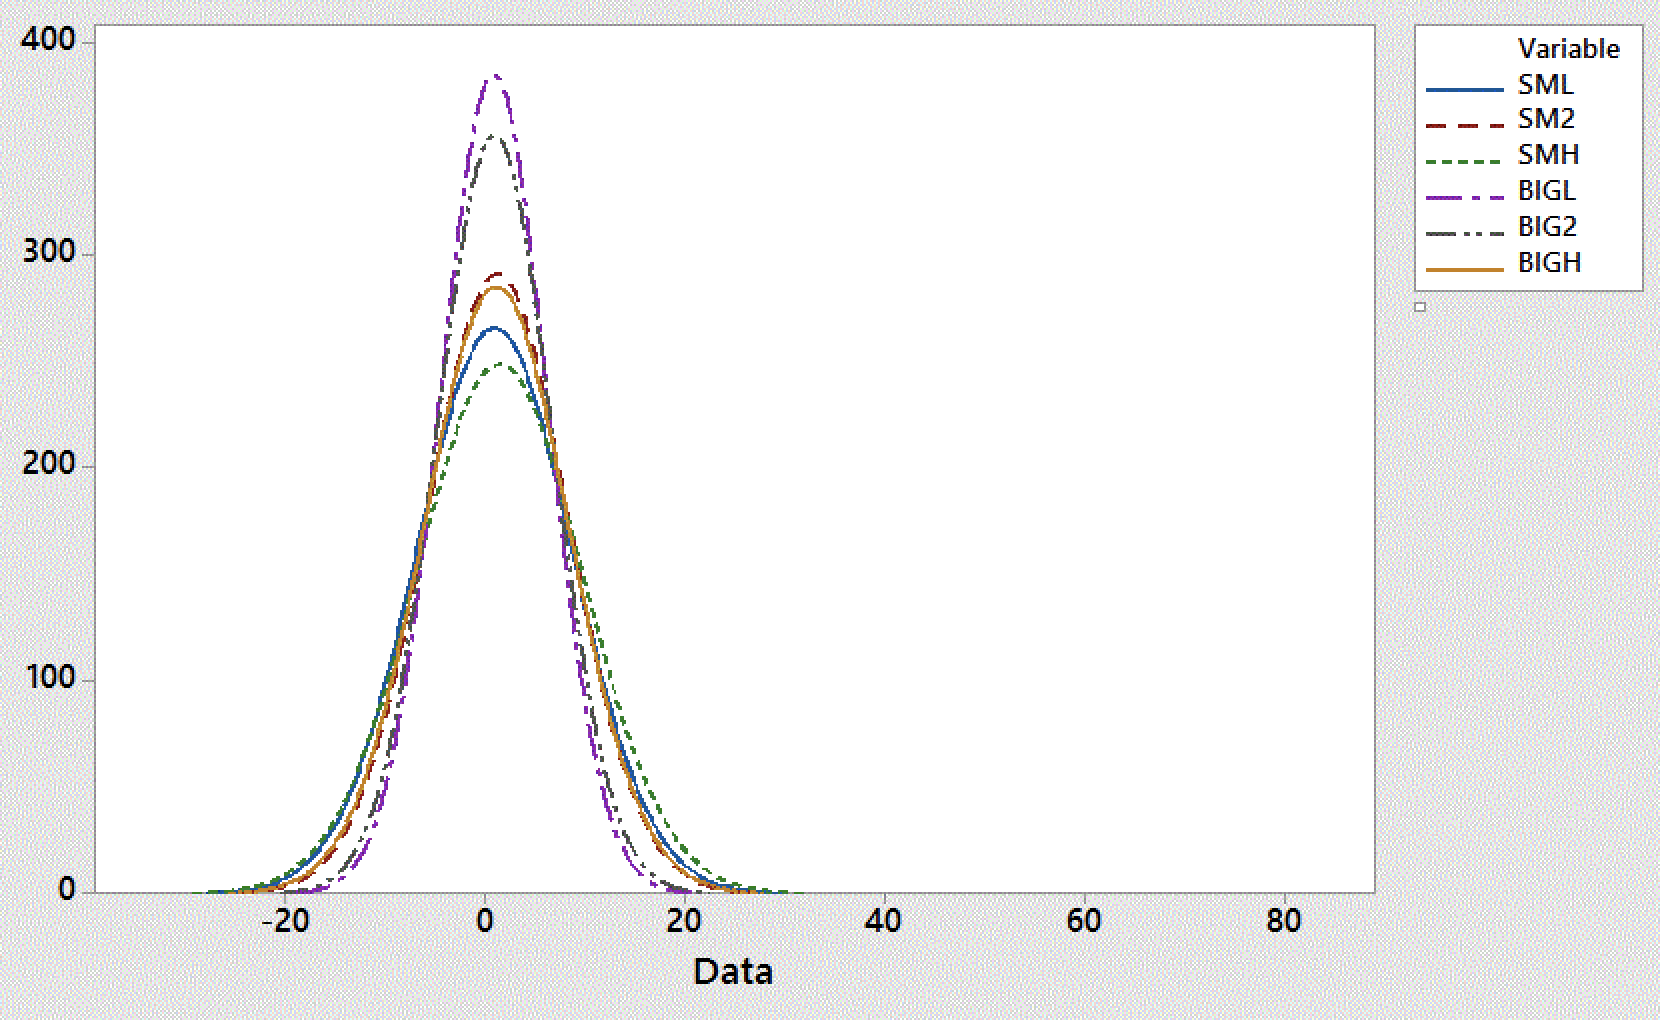
\includegraphics[width=\textwidth]{chapters/chapter_apm/figures/monreturns.png} 
	\caption{Histogram of Monthly Returns. \label{fig:monreturns}}
        \end{figure}
        
        \begin{figure}[!ht]
	\centering
	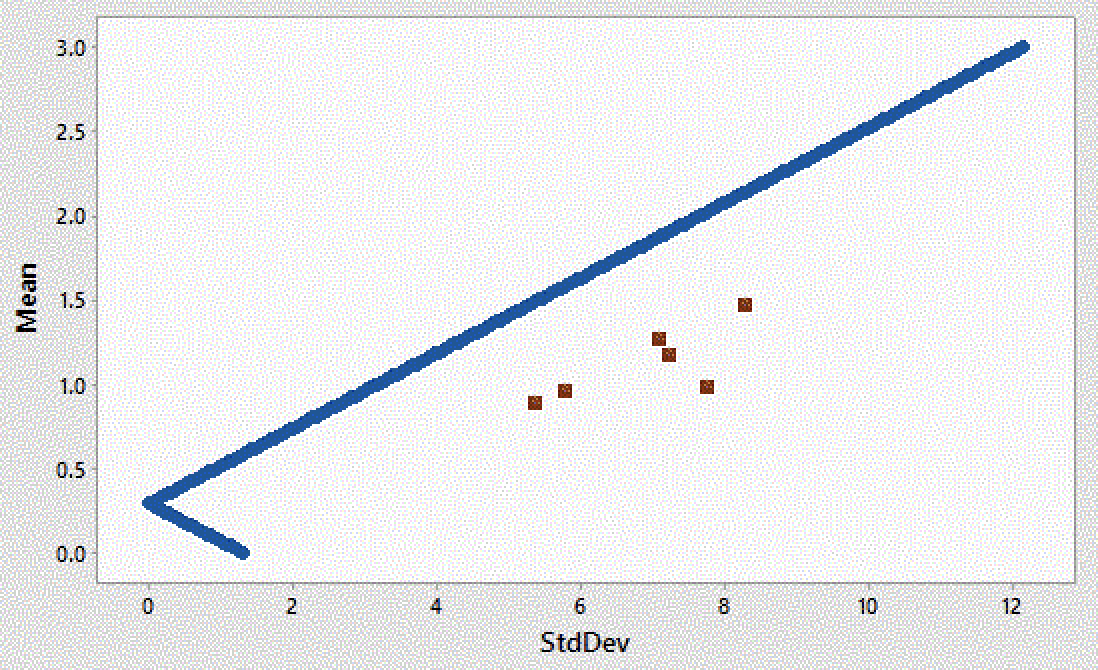
\includegraphics[width=\textwidth]{chapters/chapter_apm/figures/frontieremp.png} 
	\caption{Efficient Frontier-Empircal.\label{fig:frontemp}}
        \end{figure}
        
        \begin{table}[!ht]
        \centering
        \caption{Descriptive statistics ($T=1036$)\label{tab:descstat}}
        \begin{tabular}{lrrrrr}
        Variable & Mean & StDev & Median & Skewness & Kurtosis \\
        SML & 0.983 & 7.771 & 1.100 & 0.98 & 10.23 \\
        SM2 & 1.271 & 7.092 & 1.530 & 1.27 & 14.51 \\
        SMH & 1.472 & 8.303 & 1.660 & 2.13 & 21.64 \\
        BIGL & 0.892 & 5.365 & 1.195 & $-0.13$ & 5.16 \\
        BIG2 & 0.960 & 5.799 & 1.225 & 1.25 & 16.82 \\
        BIGH & 1.173 & 7.243 & 1.395 & 1.53 & 18.05
        \end{tabular}
        \end{table}


The histogram of the portfolio returns is given in Figure~\ref{fig:monreturns}. The descriptive are stated in Table~\ref{tab:descstat}. The returns are generally positively skewed with more sharply peaked than the normal distribution. The Jarque-Bera test (Equation~\ref{eqn:2JB}) rejects the null hypothesis that returns are normally distributed. The efficient frontier with the risk-free rate using the weights in \eqref{eqn:5weff2} along with the portfolios is plotted in Figure~\ref{fig:frontemp}, by setting $\mu^*= \hat{\mu}_m$, the average of the market portfolio. The weights for the assets are $(-1.06, 1.08, 0.40, 0.58, -0.36, -0.32)$ and the share of the risk-free is 0.68. The scatter plot of the actual mean value versus standard deviation of the six portfolios (Figure~\ref{fig:capmarket}) yields the slope of 0.1471 which is larger empirical Sharpe ratio $\left( \frac{\overline{r}_m - r_f}{\hat{\sigma}_m} \right)$, 0.1147. This clearly indicates that the market portfolio is not mean-variance efficient. Note that while three portfolios (BigL, Big2, BigH) lie on the line, two others (SM2 and SMH) lie above the line. This generally implies that it is possible to outperform the empirical Markowitz portfolio. 

        \begin{table}
        \centering
        \caption{Fama French model (estimates)\label{tab:famafrenchmodel}}
        \begin{tabular}{lrrrrr}
        Portfolio & Const & Market & SMB & HML & $R^2$ \\ \hline
        SML & $-0.168^*$ & $1.09^*$ & $1.05^*$ & $-0.167^*$ & 0.974 \\
        SM2 & 0.0625 & $0.977^*$ & $0.818^*$ & $0.702^*$ & 0.978 \\
        SMH & 0.0202 & $1.03^*$ & $0.933^*$ & $0.783^*$ & 0.991 \\
        BIGL & $0.077^*$ & $1.02^*$ & $-0.0965^*$ & $-0.231^*$ & 0.978 \\
        BIG2 & $-0.0507$ & $0.966^*$ & $-0.122^*$ & $0.729^*$ & 0.954 \\
        BIGH & $-0.112^*$ & $1.079^*$ & 0.0205 & $0.819^*$ & 0.968
        \end{tabular}
        \end{table}


The three known factor model \eqref{eqn:arbrit} results are presented in Table~\ref{tab:famafrenchmodel}. There are several conclusions that can be drawn from this table. With the three factors, the variations in the cross-sectional returns are well-captured by these factors. The coefficients of the market factors are closer to unity indicating that the six portfolios are closely aligned with the market index. But the estimates of $\alpha$ do indicate some mixed results. The value of the test statistics in \eqref{eqn:bigF} is 5.54 which is larger than $\chi_6^2 (0.05)= 2.1$ and hence indicating that there should be some consideration to other factors.


To identify the number of factors required to capture the total variance, we perform PCA of the covariance matrix. The Scree plot is given in Figure~\ref{fig:screeplot}. The first component is responsible for 91\% of the total variance and if three components are included we can capture 98\% of the overall variance. The first factor loading is almost proportional to unit vector indicating that it can be interpreted as a market factor. It is easy to show with three factor model, the difference between $\hat{\Sigma}$ and $\hat{B}\hat{B}'+V$ is very small. This sort of parameter reduction will become useful when we deal with large number of assets, a topic that is taken up in Section~\ref{s:stat_under}.


        \begin{figure}[!ht]
        \centering
        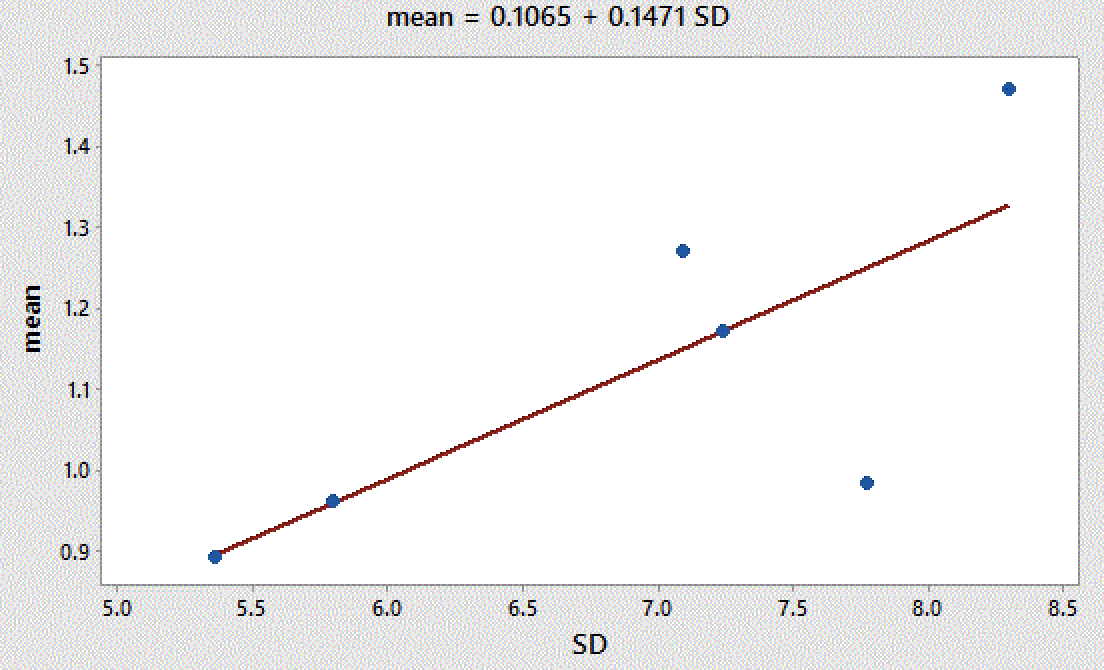
\includegraphics[width=\textwidth]{chapters/chapter_apm/figures/capmarket.png} 
        \caption{Capital Market Line.\label{fig:capmarket}}
        \end{figure}


        \begin{figure}[!ht]
        \centering
        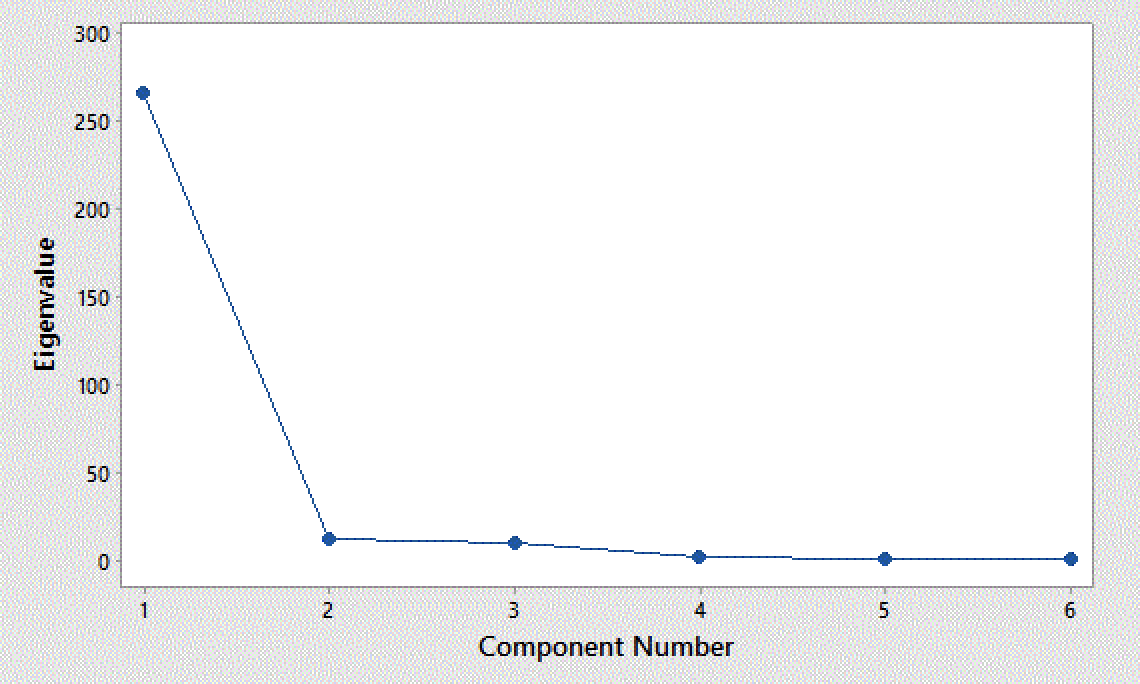
\includegraphics[width=\textwidth]{chapters/chapter_apm/figures/scree.png} 
        \caption{Scree Plot of Eigenvalues.\label{fig:screeplot}}
        \end{figure}
	


% Summary of Models and Implications for Investing	
\subsection{Summary of Models and Implications for Investing}


As the focus of this book is on trading and investing we want to summarize some main takeaways from the widely used theoretical models. Some implications of these models are listed below: \\


\noindent\textbf{One-fund Theorem:} There is a single investment of risky assets such that any efficient portfolio can be constructed as a combination of this fund and the risk-free asset. The optimal one-fund is the market fund which implies that the investor should purchase every stock which is not practical; this has given rise to the so-called index funds. \\


\noindent\textbf{Two-fund Theorem:} Two efficient portfolios (funds) can be established so that any efficient can be duplicated; all investor seeking efficient portfolios need only to invest in combinations of these two funds. \\


\noindent\textbf{No short-selling:} When the weights, $w_i$, are restricted to be positive, typically many of them tend to be zeros, by contrast with short-selling, most of the weights tend to be non-zeros. The resulting concentrated portfolios are more likely to have higher turnover rates. This has implications for the increase in trading costs. \\


\noindent\textbf{CAPM:} Recall the model is $r_i - r_f= \beta_i (r_m-r_f)+\epsilon_i$ with $\sigma_i^2= \beta_i^2\sigma^2_m + \sigma_\epsilon^2$; $\beta_i= \frac{\sigma_{im}}{\sigma_m^2}$ is the normalized version of covariance. If $\beta_i= 0$, $r_i \sim r_f$ even if $\sigma_i^2$ is large. There is no risk premium; the risk that is uncorrelated with the market can be diversified away. if $\beta_i < 0$, $r_i<r_f$ even if $\sigma_i^2$ is large; such an asset reduces the overall portfolio risk when it is combined with the market portfolio; they provide a form of insurance. Portfolio `Beta' is $\beta_p= \sum_{i=1}^m w_i \beta_i$. The CAPM can be used as a pricing formula. Note if the purchase price of an asset is `$P$' (known) which may be sold at `$Q$' (unknown), from CAPM, $r= \frac{Q-P}{P}= r_f+\beta(r_m - r_f)$ which results in the pricing formula
	\begin{equation}\label{eqn:pricing}
	P=\dfrac{Q}{1 + r_f + \beta(r_m - r_f)}.
	\end{equation}
This concept to evaluate a single asset can be extended to jointly evaluating multiple assets as well. \\


\noindent\textbf{Investment Pattern:} The minimum-variance portfolio method is likely to invest into low residual risk and low beta stocks. The CAPM model, \eqref{eqn:5ritrf} written in the vector form leads to
	\begin{equation}\label{eqn:vectorform}
	r_t - r_f 1 = \alpha + \beta(r_{mt} - r_f) + \epsilon_t
	\end{equation}
and with the assumption that the error-covariance matrix is diagonal, the covariance matrix of the excess returns is
	\begin{equation}\label{eqn:Sigmarr}
	\Sigma_{rr}= \beta\beta' \sigma_m^2 + D,
	\end{equation}	
where $D$ is diagonal with the element, $\sigma_{\epsilon i}^2$. The inverse of the covariance matrix has a simpler structure:
	\begin{equation}\label{eqn:simplestruct}
	\Sigma_{rr}^{-1}= D^{-1} - \dfrac{\sigma_m^2}{1+a} \cdot bb',
	\end{equation}	
where $a=\sigma_m^2 \cdot \sum_{i=1}^m b_i \beta_i$ and $b_i= \beta_i/\sigma_i^2$. We have shown earlier that the portfolio weights under minimum-variance is
	\begin{equation} \label{eqn:minvariance}
	w= \dfrac{\Sigma_{rr}^{-1} 1}{1' \Sigma_{rr}^{-1} 1}, \quad \sigma_{\text{MV}}^2= \dfrac{1}{1' \Sigma_{rr}^{-1} 1}.
	\end{equation}	
Substituting \eqref{eqn:simplestruct} in \eqref{eqn:minvariance}, notice that 
	\begin{equation}  \label{eqn:wsubtitute}
	w= \sigma_{\text{MV}}^2 \left( D^{-1} 1 - \dfrac{\sigma_m^2}{1+a} \cdot bb' 1\right)
	\end{equation}
with a typical element, $w_j= \frac{\sigma_{\text{MV}}^2}{\sigma_j^2} \left(1 - \beta_j \left( \frac{\sigma_m^2}{1+a} \cdot \sum_{i=1}^m b_i \right) \right)$. It is easy to show that the second term in parenthesis above, $\frac{\sigma_m^2}{1+a} \cdot \sum_{i=1}^m b_i \sim 1$ and so
	\begin{equation} \label{eqn:wsubsecond}
	w_j= \dfrac{\sigma_{\text{MV}}^2}{\sigma_j^2} ( 1- \beta_j).
	\end{equation}
Thus when $\sigma_j^2$ is small and low $\beta_j$, $w_j$ will be large. \\


\noindent\textbf{Diversifying the Diversifiers:} In practice, finding proxies for the true tangency portfolio or a completely risk-free asset has been difficult. Practitioners traditionally have used cap-weighted equity indices as proxies for tangency portfolios but that is shown to result in inefficient risk-return trade-off. Recent studies (see Amenc, Goltz, Lodh and Martellini (2012)~\cite{amencgoltzlodhmart}) focus on diversifying across various forms of efficient portfolios, notably those formed using the maximum Sharpe ratio and the minimum variance criteria. It is empirically shown that the minimum variance portfolios provide conservative exposure to stocks that perform well in adverse conditions and Sharpe ratio portfolios provide access to higher performance stocks. Combining the two with controls on tracking error results in a smoother performance. 



% Statistical Underpinnings
\section{Statistical Underpinnings \label{s:stat_under}}


The implementation of the portfolio theory in practice when the means and covariances of returns are unknown has raised some challenging issues. It is a theory that applies to a single period and the choice of portfolio weights that would determine the portfolio returns for a future period. Because of uncertainty involved in the future returns the use of the estimates of the means and covariances of the returns based on the past data must be carefully evaluated. The sample average and the sample covariance matrix (which are also maximum likelihood estimates under the assumptions that returns are normally distributed) when plugged in, the main thesis that the combination of the assets would yield efficient portfolio does not seem to hold empirically. 


The following numerical illustration taken from Bruder, Gaussel, Richard and Roncalli (2013)~\cite{bruder} is quite telling. Consider the universe of four assets with the average return vector and the covariance matrix as given below.
	\begin{equation} \label{eqn:ovrsighat}
	\begin{split}
	\overline{r}'&= (0.05, 0.06, 0.07, 0.08) \\
	\hat{\Sigma}&=\begin{pmatrix}
	0.01 & 0.0084 & 0.0098 & 0.0105 \\
	        & 0.0144 & 0.01176 & 0.0126 \\
	        &             & 0.0156 & 0.0147 \\
	        &             &             & 0.0225
	\end{pmatrix}
	\end{split}
	\end{equation}
If the risk tolerance parameter `$\lambda$' is set at 0.1, then the resulting optimal portfolio has the following weights: $w^*= (0.2349, 0.1957, 0.1878, 0.2844)$. If the standard deviation (volatility) of the second asset increases by 3\%, the weight attached to this asset changes to $-0.1404$ and if the return of the first asset changes from 5\% to 6\%, the optimal weight goes to 0.6319 from 0.2349. The sensitivity of the efficient portfolio weights even to minor perturbations is quite obvious. 


This may be due to a number of factors. We have to keep in mind that the performance of the portfolio depends on the future means and covariances of the returns. As seen from the plot of the six portfolio returns, Figure~\ref{fig:monreturns}, the distributions may not follow normal distributions. There are portfolios which are linear combinations of several individual assets and therefore individual assets can even more easily deviate from normality. Secondly, this could be result of curse of dimensionality. When `$m$' the number of assets is fairly large, the number of unknown parameters, $m(m+1)/2$ is also large and to estimate them accurately, it requires to have a fairly large data. An extreme example would be tracking Russell index with 3000~stocks would require estimating 4.5~million covariances. Another aspect that needs to be looked into is regarding the time dependence of the returns. Under efficient market hypothesis, returns are expected to be independent; but as seen in previous chapters that there is some dependence, an anomaly exploited by the algorithms, need to be taken into account in the portfolio construction. We address these issues in this section. 


It has been shown that because of the large sampling error of the estimates, an equally weighted portfolios can perform closer to the efficient portfolio. Studies have incorporated the estimation risk via Bayesian approach and evaluated the impact of this risk on final choice of the portfolios. The exact distribution of the maximum likelihood estimators of the means and variance is well-known, but the exact distribution of the returns and the volatility of the efficient portfolio is not easy to obtain. Jobson and Korkie (1980)~\cite{jobkor} derive the asymptotic distribution and examine its properties via extensive simulations. The convergence of the sample estimates is shown to depend upon the magnitude of $T$ to $1/A^2$, where $A=1' \Sigma^{-1}\mu$, the sum of weighted averages. Generally if the covariances among the assets are relatively small but the mean returns are large, the estimators tend to perform better. In any case, good estimates of `$\mu$' and `$\Sigma$' are essential for the construction of the efficient portfolio. Michaud (1989)~\cite{michaud} suggests bootstrap methods to repeatedly resample with replacement from the observed sample of returns $(r_1, \ldots, r_m)$ and use the resulting average and the variance as the the bootstrap replications. \\


\noindent\textbf{Shrinkage and Bayesian Methods:} The shrinkage methods follow the same optimization criterion but impose a penalty on the size of the coefficients. For example, we can add following additional constraints to \eqref{eqn:5opt}:
	\begin{equation} \label{eqn:addconstraint}
	\text{Ridge: } \sum_{i=1}^m w_i^2 \leq w, \qquad \text{Lasso: } \sum_{i=1}^m |w_i| \leq w.
	\end{equation}
Both procedures can be unified as, $\sum_{i=1}^m |w_i|^q \leq w$ for $1 \leq q \leq 2$. As it has been shown that these methods yield estimates that are Bayes estimates with different priors. We will now discuss Bayesian approach. 


The Bayesian approach combines the prior distribution and the likelihood to obtain posterior distribution of the unknown parameters. Usually the mode of this distribution is taken as a reasonable estimate. In a influential paper, Black and Litterman (1992)~\cite{blacklit} describe the need for Bayesian approach. The straight solution to \eqref{eqn:5opt} almost always results in large short positions in many assets which would increase the trading costs. If the weights are restricted to be positive the solution results in zero weights for many assets and large weights in the assets with small capitalizations. The results generally are not reasonable mainly due to poor estimate of expected future returns. In practice, investors augment their views using their prior experience and their intuition to forecast the likely returns based on other asset related data. The Bayes Theorem in a natural way combines these two aspects. The details that follow are from Lai, Xin and Chen (2011)~\cite{laixingchen} and we will comment on the practical implementation issues after presenting mathematical results. 


The model begins with the following distributions:
	\begin{equation} \label{eqn:5distributions}
	r_t \sim N(\mu,\Sigma), \quad \mu \big| \Sigma \sim N(\nu, \Sigma/\kappa) \text{ and } \Sigma \sim IW_m(\psi,n_0),
	\end{equation}
where $I W_m(\psi,n_0)$ is the inverted Wishart with `$n_0$' degrees of freedom with $E(\Sigma)= \psi/(n_0 - m - 1)$ (for details on invented Wishart, see Anderson (1984)~\cite{andersontw2}). These priors are known as conjugate priors as their functional forms closely match the likelihood functional form. When the degree of freedom `$\kappa$' goes to zero, the prior is non-informative. The posterior estimates are:
	\begin{equation}\label{eqn:5posterior}
	\begin{split}
	\hat{\mu}&= \dfrac{\kappa}{T+\kappa} \cdot \nu + \dfrac{T}{T+\kappa} \overline{r} \\
	\hat{\Sigma}&= \dfrac{\psi}{T+n_0-m-1} + \dfrac{T}{T+n_0-m-1} \cdot \left\{s+ \dfrac{\kappa}{T+\kappa} (\overline{r}-\nu)(\overline{r}-\nu)' \right\},
	\end{split}
	\end{equation}
where $S= \frac{1}{T} \sum_{t=1}^T (r_t - \overline{r})(r_t - \overline{r})'$, the residual covariance matrix. If `$\kappa$' and `$n_0$' are taken to be large, it implies that the investor puts more emphasis on priors. To use \eqref{eqn:5posterior}, the investor has to specify these values. 


Black and Litterman (1992)~\cite{blacklit} propose shrinking the prior estimate of $\mu$ to a vector `$\pi$' representing excess equilibrium returns such as the one implied by CAPM which is termed as the return on the global market. Thus
	\begin{equation} \label{eqn:bigpi}
	\pi = \dfrac{\mu_m-r_f}{\sigma_m^2} \cdot \Sigma \cdot w_m,
	\end{equation}
where $w_m$ are the weights on the global market and $\sigma_m^2$ is the variance of the rate of return on the global market. To get the posterior distribution of $\mu \big| \pi$ via Bayes Theorem, as mentioned in Satchell and Snowcraft (2000)~\cite{snow}, the approach by Black and Litterman (1992)~\cite{blacklit}  was to place this in a tractable form that investors can operationalize. Assume that $k \times m$ matrix $P$ represents investor's beliefs, then $P \mu \sim N(q,\Omega)$, where `$\Omega$' is diagonal. The parameters `$q$' and `$\Omega$' are known as hyperparameters. Also it is assumed that $\pi \big| \mu \sim N(\mu,\tau \Sigma)$, where $\tau$ is a scaling factor. Thus the p.d.f. of `$\mu$' is given as $\mu \big| \pi \sim N(\hat{\mu}^{\text{BL}}, \hat{\Sigma}^{\text{BL}})$, where 
	\begin{equation} \label{eqn:bleq}
	\hat{\mu}^{\text{BL}}= (\hat{\Sigma}^{\text{BL}})^{-1} [ (\tau \Sigma)^{-1}\pi + P' \Omega^{-1}q], \quad \hat{\Sigma}^{\text{BL}}= (\tau \Sigma)^{-1} + P' \Omega^{-1}P.
	\end{equation}
For various interesting practical applications, see Satchell and Snowcraft (2000)~\cite{snow}. But the requirement for subjective judgements makes it difficult to use Black-Litterman model in asset management practice. 


It has been noted in the literature that estimating the expected returns using the past returns fails to account for likely changes in the level of market risk. Merton (1980)~\cite{merton} based on a detailed exploratory study concludes that the investors should recognize that the expected market return in excess of risk free return should be positive and that there is heteroscedasticity in the realized returns. It must be noted that the price series is random walk and therefore with shifting means, the successive differences (essentially the returns) can exhibit different levels of variances. Predicting future returns under the random walk model for price is still an open issue.


Recent focus has been on the improved estimation of the covariance matrix, $\Sigma$. As the sample covariance matrix with $m(m+1)/2$ elements requires substantially large `$T$' for estimation, alternatives for a structural covariance matrix with fewer parameters are proposed. There are all in the same spirit of shrinkage estimators:
	\begin{equation} \label{eqn:5HatSigma}
	\hat{\Sigma}= \alpha s_0 + (1 - \alpha) s,
	\end{equation}
where `$\alpha$' is called a shrinkage constant and `$s_0$' matrix is restricted to have only a few `freer' elements. With the CAPM model that leads to covariance structure, \eqref{eqn:Sigmarr}, the resulting covariance matrix which is the sum of a diagonal matrix and a matrix of rank one, will have only `$2m$' independent elements that need to be estimated. Ledoit and Wolf (2003)~\cite{wolf} describe a procedure to arrive at the estimate of $\alpha$ in \eqref{eqn:5HatSigma}, which we briefly describe below. 


Minimizing the following risk function,
	\begin{equation} \label{eqn:ralpha}
	R(\alpha)= \sum_{i=1}^m \sum_{j=1}^m E(\alpha s_{ij}^0 + (1-\alpha) s_{ij} - \sigma_{ij})^2,
	\end{equation}
we arrive at `$\alpha$' as
	\begin{equation}\label{eqn:bigalpha}
	\alpha^*= \dfrac{\sum_i \sum_{j} \left[ \Var(s_{ij}) - \cov(s_{ij}^0, s_{ij}) \right]}{\sum_i \sum_j \left[ \var(s_{ij}^0 - s_{ij}) + (\phi_{ij} - \sigma_{ij})^2 \right]},
	\end{equation}
where $\phi_{ij}= E[\alpha s_{ij}^0 + (1 - \alpha) s_{ij}]$. It is further shown that
	\begin{equation}\label{eqn:alphastarsim}
	\alpha^* \sim \dfrac{1}{T} \cdot \dfrac{\pi - \rho}{\gamma},
	\end{equation}
where $\pi= \sum_i \sum_j \text{Asy} \var(\sqrt{T} s_{ij})$, $\rho= \sum_i \sum_j \text{Asy} \cov(\sqrt{T}\,s_{ij}^0, s_{ij})$ and $\gamma= \sum_i \sum_j (\phi_{ij} - \sigma_{ij})^2$. Note that with CAPM specification which can be taken as a single index model, the `$\gamma$' quantity represents the misspecification of the single index. 


Fan, Fan and Lv (2008)~\cite{fansq} consider high dimensional covariance matrix estimation via factor model \eqref{eqn:arbrit}. The multifactor model generally captures well the cross-sectional variations and thus the number of parameters that need to be estimated can be significantly reduced. It is possible that the number of factors `$n$' can grow with the number of assets, `$m$', and the sample period, `$T$'. Comparing $\hat{\Sigma}_{rr}= \hat{B} \hat{\Omega} \hat{B}' + \hat{V}$ in \eqref{eqn:covdouble} with the sample covariance matrix of the returns, `$S$', it is shown that the former performs better if the underlying factor model is true. In calculations that involve the inverse of the covariance matrix, such as the calculation of portfolio weights, factor model based estimates tend to perform better but it does not make a difference in the actual risk calculation $(\hat{w}' \hat{\Sigma} \hat{w})$, which involves the estimate of the covariance matrix. Recent studies have focused on proving bounds on the risk; the calculations are somewhat complicated as they involve estimates of the weight vector as well as the estimates of the covariance matrix. See Fan, Han, Liu and Vickers (2016)~\cite{vickers} and the references therein for additional details.



% Portfolio Allocation Using Regularization
\subsection{Portfolio Allocation Using Regularization}


It is noted that the poor performance of Markowitz's conceptual framework is due to the structure of the optimization problem. It is an ill-conditioned inverse problem as the solution requires the inverse of the covariance matrix that may involve highly correlated securities. A number of regularization procedures have been proposed in the literature to address the instability in the solution and we present a few of them here. \\


\noindent\textbf{The $\mathbf{L_2}$ Constraint:} This is also known as ridge constraint that imposes the penalty on the size of the estimates as given in \eqref{eqn:addconstraint}. The problem is defined as follows:
	\begin{equation} \label{eqn:minwsum}
	\min_w w' \Sigma w \ni w' \mu= \mu^*, w'\mu= 1 \text{ and }\sum_{i=1}^m w_i^2 \leq w_0
	\end{equation}
when there are many correlated assets, the weights are poorly determined and can exhibit high variance. A large positive weight for an asset can be canceled by a large negative weight for the correlated asset. The size constraint added in \eqref{eqn:minwsum} can address this issue. If the added constraint has the associated Lagrangian multiplier, $\gamma^*$, the solution in \eqref{eqn:5weff} is modified by replacing $\Sigma$ by ($\Sigma + \gamma^* I_m$). The solution adds a positive constant to smaller eigenvalues of possibly a singular matrix, $\Sigma$. Observe that the eigenvalue decomposition of $\Sigma= V \Lambda V'$ essentially gives us the principal components of the asset universe considered for the formation of the portfolio. The optimization can also be extended to accommodating to mimic a target portfolio with weights $w^*$. The set-up would be the same except for the last size constraint is replaced by
	\begin{equation} \label{eqn:wminwstar}
	(w - w^*)' A(w - w^*) \leq w_0,
	\end{equation}
where $A$ is a general specified matrix. If `$\lambda$' and `$\gamma$' are the Lagrangian multipliers associated with the mean specification constraint in \eqref{eqn:wminwstar} and the constraint above, the solution is
	\begin{equation} \label{eqn:hatwlambdagamma}
	\hat{w}(\lambda,\gamma)= (\hat{\Sigma} + \gamma A)^{-1} (\lambda \hat{\mu} + \gamma A w_0),
	\end{equation}
which results from shrinking both the mean vector and the covariance matrix. \\


\noindent\textbf{The $\mathbf{L_1}$ Constraint:} The shrinkage method LASSO (least absolute shrinkage and selection operator) is like the ridge method (see \eqref{eqn:addconstraint} above) but there are some important differences. The problem can be stated as follows:
	\begin{equation} \label{eqn:minwsum2}
	\min_w w' \Sigma w \ni w'\mu=\mu^*, w'\mu=1 \text{ and } \sum_{i=1}^m |w_i| \leq w_0
	\end{equation}
The added constraint in \eqref{eqn:minwsum2} leads to nonlinear solutions and no explicit solution as with ridge penalty is possible. The numerical solutions are obtained via quadratic programming.


Both $L_1$ and $L_2$ constraint versions yield solutions that can be justified as Bayes with different priors. The LASSO method produces sparse solution that is easy to interpret. Sparser solution in the portfolio context means lower transaction costs when the portfolios are rebalanced. A convenient way to solve these optimization problems is to formulate the original set-up in \eqref{eqn:5opt} in the regression framework; this will help to borrow regularization ideas used in the general area of multivariate regression. Observe that $\Sigma= E(r_tr_t') - \mu\mu'$ and thus the minimization problem is equivalent to (in the sample version)
	\begin{equation} \label{eqn:hatwarg}
	\hat{w}= \text{arg }\min_w \dfrac{1}{T} \| \mu^*1_T - R'w\|_2 \ni w'\hat{\mu} = \mu^*, w'1_m=1.
	\end{equation}
Here, $R$ is the $m\times T$ matrix of the row returns and $\hat{\mu}=\frac{1}{T}\sum_{t=1}^T r_t$. The regularization constraint in \eqref{eqn:minwsum2} when added to \eqref{eqn:hatwarg} results in the following optimization problem:
	\begin{equation}\label{eqn:anotherhatwargmin}
	\hat{w}^{(\tau)}= \text{arg } \min_w [ \|\mu^* 1_T - R'w\|_2 + \tau\|w\|_1] \ni w' \hat{\mu} = \mu^*, w'1_m=1.
	\end{equation}
As stated in Brodie, Daubechies, De Mol, Giannone and Loris (2009)~\cite{brodic} adding the $L_1$-constraint results in several useful advantages. In addition to introducing sparsity that is helpful for managing large portfolios, the procedure provides a framework for regulating the amount of shorting which can be a proxy for the transaction costs. More importantly it provides a solution that is more stable which was a main concern in the original optimization set-up as small perturbations in the estimates of $\mu$ and $\Sigma$ can lead to very different solutions.


The algorithm that is most convenient to solve \eqref{eqn:anotherhatwargmin} is Least Angle Regression (LAR) developed in Efron, Hastie, Johnstone and Tibshirani (2004)~\cite{efron}. It starts with a large value of `$\tau$' in \eqref{eqn:anotherhatwargmin} and as `$\tau$' decreases the optimal solution, $\hat{w}^{(\tau)}$, changes in a piecewise linear fashion and thus it is only essential to find critical points where the slope changes. More relevant details can be found in Brodic et al. (2009)~\cite{brodic}. The LASSO procedure was evaluated using Fama-French 100 portfolios sorted by size and book-to-market as the universe. The efficient portfolio was constructed on a rolling basis using the monthly data for five years and its performance is evaluated in the following year. It is concluded, see Brodie et al. (2009; Figure 2)~\cite{brodic}, that optimal sparse portfolios that allow short portfolios tend to outperform both optimal no-short-positions portfolio and the na\"ive evenly weighted portfolio. 



% Portfolio Strategies: Some General Findings
\subsection{Portfolio Strategies: Some General Findings}


The following wisdom advocated by Rabbi Isaac bar Aha that ``one should always divide his wealth into three parts: a third in land, a third in merchandise and a third ready to hand'', the equal division among the assets has been tested out in the case of equity allocation as well. Although this diversification strategy appears to be na\"ive because it is based on neither any theory nor any data, has done relatively well and has stood out as a folk wisdom. DeMiguel, Garlappi and Uppal (2009)~\cite{demig} compare this na\"ive strategy with other theory-based strategies that were discussed in earlier sections in terms of its performance using various data sets. The summary of their findings is worth noting: ``\dots of the strategies from the optimizing models, there is no single strategy that dominates the $1/N$ strategy in terms of Sharpe ratio. In general, $1/N$ strategy has Sharpe ratios that are higher \dots relative to the constrained policies which in turn have Sharpe ratios that are higher than those for the unconstrained policies.''


The na\"ive portfolio has also very low turnover. In addition to keeping na\"ive portfolio as  a benchmark, a practical implication is that the estimation of the moments of asset returns needs improvement using other information based on asset characteristics. \\


\noindent\textbf{Combination of Strategies:} Tu and Zhou (2011)~\cite{jtu} combine the rules based on Markowitz Theory with the na\"ive strategy to obtain new portfolio rules that can perform uniformly better. The combination can be interpreted as a shrinkage estimator, shrinking toward the na\"ive estimator. The linear combination
	\begin{equation} \label{eqn:lincomb}
	\hat{w}_c = \delta \hat{w} + (1-\delta) w_N,
	\end{equation}
where $\hat{w}$ is the weights that come from variations of efficient portfolios and $w_N$ has all its elements equal. With the criterion of minimizing the loss function, 
	\begin{equation} \label{eqn:lossfun}
	L(w^*,\hat{w}_c)= U(w^*) - E[U(\hat{w}_c)],
	\end{equation}
where $U(\cdot)$ is the expected utility, the combination coefficient $\delta$, is obtained. This strategy was tested out using the same data as in DeMiguel et al. (2009)~\cite{demig} and generally the combination rules perform well. This idea is in the same realm as diversification of diverse strategies. \\


\noindent \textbf{Familiarity:} It has been advocated by many economists and practitioners such as Warren Buffet that investors should focus on a few stocks that they are familiar with rather than a wide scale diversification. Boyle, Garlappi, Uppal and Wang (2012)~\cite{bguwang} develop a theoretical framework to answer some relevant questions related to familiarity and diversification. Writing the return as sum of components, systematic and idiosyncratic,
	\begin{equation} \label{eqn:rirsui}
	r_i = r_s + u_i \quad\quad i= 1, 2, \ldots, m
	\end{equation}
the utility function in \eqref{eqn:utility} is modified to take into account the investors familiarity with some assets. This is done via the assumption that the investor is ambiguous about the mean, $\mu$, but has perfect knowledge about $\sigma$. This information alters the criterion in \eqref{eqn:5maxu} as,
	\begin{equation}\label{eqn:maxminwmu}
	\max_w \min_\mu \left( w'\mu - \frac{\lambda}{2} \cdot w' \Sigma w \right) \enskip \ni \enskip \dfrac{(\mu-\hat{\mu})^2}{\sigma_{\hat{\mu}}^2} \leq \alpha_i^2, \quad i= 1, 2, \ldots, m,
	\end{equation}
where $\sigma_{\hat{\mu}}^2= (\sigma_s^2+\sigma_u^2)/T$. Two key quantities that play important roles are the level of ambiguity `$\alpha_i$' and the inverse coefficient of variation, $\hat{\mu}/\sigma_{\hat{\mu}}$. Some conclusions from this study are, when ambiguity is present, the investor tends to hold disproportionate (to Markowitz allocation) amount in the familiar assets and the number of assets tends to be smaller.


Huberman (2001)~\cite{Hub} provides several instances of investment in the familiar options rather than choices that lead to efficient outcome. Workers generally tend to choose their employer's stock as they probably think that they know about their behavior and may believe they have information that the market does not have. Thus various examples are provided that indicate that although investment in the familiar stocks contradicts the advice to diversify. This adds a dimension to the traditional risk-return formulation that one has to recognize. \\


\noindent\textbf{Large Portfolio Selection with Exposure Constraints:} Several techniques have been discussed in this section to reduce the sensitivity of the optimal portfolio weights to uncertainty in the inputs, such as the mean returns and the covariance matrix of returns. Generally these techniques are not adequate to address the effect of estimation errors that accumulate due to large portfolio size. Jagannathan and Ma (2003)~\cite{jagma} impose no short-sales constraints as well as upper bounds on portfolio weights as commonly imposed by practitioners. The empirical evidence indicates that simply imposing upper bounds does not lead to significant improvement in the out-of-sample performance. For an estimated covariance matrix, $S$, the formulation of the model is as follows:
	\begin{equation} \label{eqn:estcovmat}
	\min_w w'Sw \enskip \ni \enskip w'1=1, \enskip 0\leq w_i \leq \tilde{w} \enskip\text{ for }i= 1, 2, \ldots, m.
	\end{equation}
Note the variation in its formulation; no expectation on the average return of the portfolio as in Markowitz set-up is specified. Fan, Zhang and Yu (2012)~\cite{fanzhanyu} argue that the resulting optimal portfolio, although performs well, it is not diversified enough. 


Defining the total proportions of long and short positions by $w^+=(\|w\|_1+1)/2$ and $w^-= (\|w\|_1-1)/2$, we have $w^+ + w^-= \|w\|_1$ and $w^+ - w^- =1$. The optimization problem is stated as,
	\begin{equation} \label{eqn:optproblem}
	\max_w E[U(w'r)] \enskip \ni \enskip w'1=1, \|w\|_1 \leq C \text{ and } Aw=a.
	\end{equation}
Here $U(\cdot)$ is a utility function and the extra-constraints $Aw=a$ can capture allocations to various sectors. But the key added constraint, $\|w\|_1 \leq C$ can accommodate from no short sales ($C=1$) to unrestricted sales ($C= \infty$) constraints. The solution to \eqref{eqn:optproblem} can be obtained via quadratic programming. Fan et al. (2012)~\cite{fanzhanyu} advocate data-driven choice of `$C$' via minimizing the risk for a sample learning period. Using select 600 stocks from the pool of stocks that constitute Russell 3000, the constructed portfolios tend to perform well for $C \sim 2$. 



% Dynamic Portfolio Selection
\section{Dynamic Portfolio Selection}


The static Markowitz framework, as discussed in the last section, is not realistic for practical implication. Dynamic approaches that have been discussed in the literature will be presented here briefly. The single period optimization problem can be formulated as,
	\begin{equation} \label{eqn:periodopt}
	\max_{w_t} E_t \left[ w_t' r_{t+1} - \frac{\gamma}{2}(w_t' r_{t+1})^2 \right]
	\end{equation} 
which results in the optimal solution,
	\begin{equation} \label{eqn:periodoptimal}
	w_t= w= \frac{1}{\gamma} \cdot E \left[r_{t+1} r_{t+1}']^{-1} E[r_{t+1} \right]
	\end{equation}	
that can be estimated using the sample counterpart. Here $r_{t+1}$ is taken to be the excess returns $R_{t+1} - R_t^f$. It is assumed here that the returns are independent and identically distributed. Brandt and Santa-Clara (2006)~\cite{bransc} extend the above set-up to multiperiods. Simply stated the two-period mean-variance objective function is,
	\begin{equation} \label{eqn:twoperiodmv}
	\max E_t \left[ r^p_{t \to t+2} - \frac{\gamma}{2} ( r^p_{t \to t+2})^2 \right],
	\end{equation}
where the excess return for the two period investment strategy is,
	\begin{equation} \label{eqn:twoperexcess}
	r^p_{t \to t+2} = (R_t^f + w_t' r_{t+1}) ( R^f_{t+1} + w_{t+1}' r_{t+2}) - R_t^f R_{t+1}^f.
	\end{equation}	
It can be seen that the above expression can be written as 
	\begin{equation} \label{eqn:rewritten}
	r^p_{t \to t+2} = w_t' (r_{t+1} R_{t+1}^f) + w_{t+1}' (r_{t+2}R_t^f) + (w_t' r_{t+1})(w_{t+1}' r_{t+2})
	\end{equation}
with the first two terms denoting excess returns from investing in the risk free asset in the first period and in the risky asset in the second period and vice versa. The third term that captures the effect of compounding is of smaller magnitude. Ignoring that term results in the optimal portfolio weights,
	\begin{equation}\label{eqn:optimalweights}
	w= \frac{1}{\gamma} E\left[ r^{p}_{t \to t+2} {r'}^p_{t\to t+2} \right] E[r^{p}_{t \to t+2}].
	\end{equation}
The solution reflects the the choice between holdings the risky assets in the first period only and holding them in the second period only and thus is termed as ``timing portfolios''. The above result can be extended to any number of periods. \\


\noindent\textbf{Conditioning Information in Portofolio Construction:} It has been debated that the portfolio managers may use conditioning information they have about assets in forming the portfolios, not simply using the mean and variance of the past returns. Thus the managers' conditionally efficient portfolios may not appear efficient to the investor with no knowledge of that information. Ferson and Siegel (2001)~\cite{fersie} study the properties of unconditional minimum-variance portfolios when the conditioning information is present and suggest that, ``For extreme signals about the returns of risky assets, the efficient solution requires a conservative response.'' Managers can reduce risk by taking a small position in the risky asset while keeping the same level of portfolio performance. In its basic formulation, assuming that the investment alternatives are a risky asset and risk-free return, with $w(\tilde{S})$---the proportion invested in the risky-asset, the portfolio return and the variance are: 
	\begin{equation} \label{eqn:preturnvar}
	\mu_p= E[r_f+w(\tilde{S})(r_t-r_f)], \quad \sigma_p^2= E[(w(\tilde{S})(r_t - r_f))^2] - (\mu_p - r_f)^2.
	\end{equation}
Here $\tilde{S}$ is the observed signal and $w(\tilde{S})$ is a function of that signal that the manager considers at the time of allocation. The minimization criterion leads to the following weight for the risk asset:
	\begin{equation} \label{eqn:riskyassetweight}
	w(\tilde{S})= \dfrac{\mu_p - r_f}{C} \left( \dfrac{\mu(\tilde{S}) - r_f}{(\mu(\tilde{S} - r_f)^2 + \sigma^2_\epsilon(\tilde{S})} \right),
	\end{equation}
where $C= E\left[ \frac{(\mu(\tilde{S}) - r_f)^2}{(\mu(\tilde{S}) - r_f)^2 + \sigma^2_\epsilon(\tilde{S})} \right]$ and the minimized variance is ${\sigma_p^2=(\mu_p - r_f)^2 \left( \dfrac{1}{C} - 1 \right)}$. Here $\sigma_\epsilon^2(\tilde{S})$ is the conditional variance given the signal. Note when this is zero, which signifies that there is no conditional information, $w(\tilde{S})= w= (\mu_p - r_f)/(\mu - r_f)$, that is the result of Markowitz theorem. The above results can be easily extended to multiple risky asset scenario.


To implement this idea, we assume that the weight vector is a linear function of `$k$' state variables:
	\begin{equation} \label{eqn:statevar}
	w_t= \theta z_t
	\end{equation}
and the maximization criterion in \eqref{eqn:periodopt} can be modified as,
	\begin{equation} \label{eqn:prevmodified}
	\max_\theta E_t\left[(\theta z_t)' r_{t+1} - \frac{\gamma}{2}(\theta z_t)' r_{t+1} r_{t+1}' (\theta z_t)\right].
	\end{equation}
Denoting $\overline{r}_{t+1}= z_t \otimes r_{t+1}$ and $\tilde{w}= \tvec(\theta)$, we can obtain the optimal solution as,
	\begin{equation} \label{eqn:modifiedsolution}
	\tilde{w}= \frac{1}{\gamma} E[\tilde{r}_{t+1} \tilde{r}_{t+1}']^{-1} E(\tilde{r}_{t+1})= \frac{1}{\gamma} E[(z_t z_t') \otimes (r_{t+1}r_{t+1}')]^{-1} E[z_t \otimes r_{t-1}].
	\end{equation}
Here $\otimes$ is meant for a Kronecker product. Brandt and Santa-Clara (2006)~\cite{bransc} also show how both single period and multi-period problems can be formulated as the constrained VAR. 


Using the established evidence from the literature that market returns can be predicted by conditioning on dividend-price ratio, short-term interest rate, term spread and credit spread, to study the market returns for both stocks and bonds, the authors evaluate the conditional and unconditional policies at monthly, quarterly and annual holding periods, with the value of $\gamma= 5$. Some general conclusions are:
	\begin{enumerate}[--]
	\item Conditional policies are quite sensitive to state variables. Because of the predictability of returns, conditional policies allow for the investor to be more aggressive on average. Sharpe ratios are generally higher for conditional policies.
	\item Results are less pronounced for the longer holding periods. Conditional policies can be very different at different time frequencies. 
	\end{enumerate}
The above stated conclusions hold for multi-period portfolio policies as well with monthly rebalancing. 



% Portfolio Tracking and Rebalancing
\section{Portfolio Tracking and Rebalancing}


The proportions of capital allocated to various assets can change due to their performances and investors risk aversion or objectives also can change over time. Thus, investors often engage in portfolio rebalancing to keep the portfolio on target risk exposure and exploit the market opportunities to enhance returns in the long run. First, we formulate the problem with constraints that account for these and then present the results of some empirical studies.


The portfolio returns ($r_t$) are generally compared with some index returns ($I_t$); the excess return (ER) are the tracking error (TE) are defined as follows:
	\begin{equation} \label{eqn:excesstrack}
	\text{ER}= \dfrac{1}{T} \sum_{t=1}^T (r_t - I_t), \quad TE= \dfrac{1}{T} \sum_{t=1}^T (r_T - I_t)^2.
	\end{equation}
The optimization function is to minimize $\lambda \sqrt{\text{TE}} - (1 - \lambda) \text{ER}$, via the choice of the portfolio weights. Another optimization set-up is to balance between tracking error and transaction costs. Let $x= w - w_0$, where `$w_0$' is the current portfolio weights and `$w$' is the target weights; the problem with constraints can be stated as:
	\begin{equation} \label{eqn:constraintprob}
	\min_w (w - w_0) \Omega (w-w_0) \enskip \ni w'1= 1
	\end{equation}
subject to the following constraints:
	\begin{equation} \label{eqn:constraintlist}
	\begin{split}
	&\text{long only:} \quad w \geq 0 \\
	&\text{turn-over:} \quad \sum_{i=1}^m |x_i| \leq u \\
	&\text{maximum exposure to a factor:} \quad \sum_{i=1}^m \beta_{ik} w_i \leq u_k \\
	&\text{holding:} \quad l_i \leq w_i \leq u_i
	\end{split}
	\end{equation}
Note the criterion in \eqref{eqn:constraintprob} can also be taken as a version of tracking error. 


Some practical implementation ideas are discussed in Pachmanova and Fabozzi (2014)~\cite{pachfab}. In addition to na\"ive allocation strategy discussed earlier in this chapter, other ad-hoc methods simply imitate the composition of some market indices such as S\&P 500 that weighs stocks by their market capitalizations or Dow-Jones that weighs stocks by their prices. To imitate, select the stocks with the largest weights in the benchmark. Other methods include stratification of benchmarks into groups and select stocks from each group that ensures diversification. The group can be industry-based or if it is based on past performance, the selected assets are called basis assets. The difference between the original allocation model and the rebalancing models can be due to change in the objectives and also change in the transaction costs and taxes. If a manager wants to move toward higher alpha, the restriction on the tracking error should be added to \eqref{eqn:constraintlist}. Like other calculations related to portfolio management, the rebalancing also involves backward-looking estimates. To reflect the future more accurately, managers should arrive at forward-looking estimates of tracking error using conditioning arguments given in the earlier section. \\


\noindent\textbf{Transaction Costs:} Bid-ask spreads, brokerage fees, taxes and the price impact on trading are covered in Chapter~\ref{chap:ch_mi_models}. Here we present some observations related to trading costs as noted in the literature. Defining the turnover as,
	\begin{equation} \label{eqn:turnover}
	\mathcal{T}= \sum_{i=1}^m \lvert w_i - w_{0i} \rvert = \sum_{i=1}^m \tau_i
	\end{equation}
and the costs of rebalancing is
	\begin{equation} \label{eqn:rebalance}
	C= \sum_{i=1}^m k_i \tau_i
	\end{equation}
Note $w_{0i}= \frac{w_i r_i}{\sum w_i r_i}$ and $\tau_i= \left| \frac{w_i(r_i-r_{0i})}{\sum w_ir_i} \right|$ and thus a key term here is $r_i-r_{0i}$, the difference between the actual and target return for asset `$i$'. Kourtis (2014)~\cite{kourtis} studies the distribution of $\tau$ and $C$ under the na\"ive allocation strategy. Denoting $r^p=\sum w_i r_i$ the portfolio return, the distribution of $\tau_i$ depends on $(r_i-r_{0i})/r^p$, the ratio of excess return to the portfolio return. A general criterion that accounts for the transaction cost is
	\begin{equation} \label{eqn:transcostaccount}
	\min_w \delta (w-w_0)' \Omega(w-w_0) + \sum_{i=1}^m k_i E[\tau_i (r_{i,}w)]
	\end{equation}
with the controlling parameter, $\delta$, on the tracking error. By explicitly incorporating the trading cost in the criterion, it is shown that the total cost of transaction is reduced.


Moorman (2014)~\cite{moorman} considers three portfolio strategies: a levered-momentum strategy, a zero-cost-decile momentum strategy and equally-weighted na\"ive strategy. Because the momentum strategies adapt to changing market conditions swiftly, they require frequent rebalancing and can reveal the drawbacks of any method to reduce transaction costs. First there is a no-trade region where the distance between target and the current weight is not significant. Write the rebalanced weight as,
	\begin{equation} \label{eqn:rebalanceweight}
	w_t^*= \alpha_t w_{0t} + (1 - \alpha_t)\, w_t,
	\end{equation}
where `$\alpha_t$' is the rate of rebalancing; if $\alpha_t=1$, then there is no rebalancing. It is easily seen that the current month's unbalanced weights are related to prior month's rebalanced weights as,
	\begin{equation} \label{eqn:priorrebalanced}
	w_{0t}= w_{t-1}^* \left( \dfrac{1-r_t}{1+r_{pt}} \right),
	\end{equation}
where $r_{pt}$ is the return on the portfolio before-transaction cost. Note
	\begin{equation}\label{eqn:transnote}
	r_{pt}= \sum_{i=1}^{N_t} w_{it}^* r_{it} - c_{it} \lvert w_{it}^* - w_{0t} \rvert,
	\end{equation}
where $c_{it}$ is the cost of transaction. The `$\alpha$' is chosen using the following objective function that results from constant relative risk aversion utility:
	\begin{equation}\label{eqn:objectivefun}
	\max_\alpha \dfrac{1}{T} \sum_{t=0}^{T-1} \dfrac{(1 + r_{pt+1})^{1-\gamma}}{1-\gamma},
	\end{equation}
where `$\gamma$' is the coefficient of relative risk-aversion. The parameter `$\alpha$' is chosen via grid search, outside no-trade zone. An empirical investigation of various distance and rebalancing methods reveal that transaction cost reduction is most successful for the lower momentum and equally-weighted market portfolios but more difficult for the momentum portfolios because of higher turnover. 



% Transaction Costs, Shorting and Liquidity Constraints
\section{Transaction Costs, Shorting and Liquidity Constraints}


It is clear, based on the discussion in this chapter that the managers tend to mimic better performing portfolios or use information that they have about future values of the assets in the construction and rebalancing of the portfolios. But at the end of investment horizon, the performance evaluation of the selected portfolio depends on the average returns after adjusting for the risk premia. Consider the $k$-factor models, \eqref{eqn:arbrit}, $r_{it}= \alpha_i + \beta_i' f_t + \epsilon_{it}$ and the equation that relates the average return to risk premia ($\lambda_k$), $\mu_i=r_f + \beta_i' \lambda_k$ in \eqref{eqn:mewirf}. The equation \eqref{eqn:arbrit} can be also written more compactly as,
	\begin{equation} \label{eqn:compactarb}
	r_t= \alpha + B f_t + \epsilon_t,
	\end{equation}
where $\alpha$ is a $m \times 1$ vector and $B$ is the $m \times k$ matrix of factor premia. Thus the portfolio return,
	\begin{equation} \label{eqn:portreturn1}
	r_{pt}= w'r_t = w' \alpha+ w'B f_t + w' \epsilon_t= \alpha_p + \beta_p' f_t + \epsilon_{pt}.
	\end{equation}
Because `$w$' is random, note
	\begin{equation} \label{eqn:portreturnrandom}
	E(r_{pt})= E(\alpha_p) + E(\beta_p' f_t)= \alpha' E(w)+ \Cov(\beta_p,f_t) + E(\beta_p') E(f_t).
	\end{equation}
Note the first term is the result of asset choice, the second term is the result of the factor model theory and the last term reflects the risk premia. \\


\noindent\textbf{Choice of Assets:} The screening of candidate assets relies upon assessing the underlying factor for return behavior of a portfolio. Factors are grouped into generally as fundamental factors and macroeconomic factors, although there are other considerations such as if investing in certain assets are considered to be socially responsible, or environmentally safe, etc.. Fundamental factors are related to the asset characteristics and other information such as analysts forecasts and the macroeconomic factors relate to activities in the economy that are likely to be closely associated with the asset behavior. These may be industry factors or sentiment factors. These factors can be standardized and an aggregate score can be used to sort out the assets. Several sorting methodologies are available in the literature. Using the factor scores, sort the stocks and go long on stocks with high scores and go short on stocks with low values. This method is easy to implement and it diversifies away risk of individual stocks. Some disadvantages are that it may be difficult to infer which variables provide unique information and portfolios may pick up different undesirable risks. 


Patton and Timmermann (2010)~\cite{pattim} test for positive relation between ex-ante estimates of CAPM beta and the resulting returns using daily data. Stocks are sorted at the start of each month into deciles on the basis of their betas using prior one year daily data and value-weighted portfolios are formed. Returns for these portfolios are recorded for the following month. If the CAPM holds, one should expect the average returns should increase with the betas, which is empirically confirmed. The authors also examine if the post-ranked betas of portfolios ranked by ex-ante beta estimates are monotonic confirming the predictability of the betas. Sorting the stocks based on their betas and forming decile portfolios, the performance is evaluated in the subsequent month. Specifically from the CAPM model, $r_{it}= \alpha + \beta_i r_{mt} + \epsilon_{it}$ for $i= 1, 2, \ldots, 10$, the following hypothesis, $H_0: \beta_1 \geq \beta_2 \geq \cdots \geq \beta_{10}$ is tested. The estimates range from 1.54 to 0.6 and the hypothesis is confirmed. This approach is extended to two-way sorts; firm size and book-to-market ratio or firm size and momentum. It is concluded that the size effect in average returns is absent among loser stocks. Also momentum effects are stronger for small and medium size forms. \\


\noindent\textbf{Alpha and Beta Strategies:} Portfolio managers have traditionally developed strategies to maximize `$\alpha$' in the factor model. One of the measures, information ratio defined in Chapter~\ref{ch:stat_ts} is taken as an index for the portfolios performance. But after the 2007--2008 financial crisis, there is a great deal of interest in smart-beta (referring to the coefficients of the factor model) strategies. This is a broad term that refers to from ad-hoc strategies to a mix of optimized simpler portfolios and investments in non-traditional asset classes. The construction is generally rule-based and is transparent. The commonality among them is in their exposure to factors that investors are comfortable to choose from. Kahn and Lemmon (2015)~\cite{lemmon} provide a framework to understand the beta strategies along the decomposition of return in \eqref{eqn:portreturnrandom} into three returns. To summarize:
	\begin{enumerate}[--]
	\item ``The smart-beta return arises from static (i.e. long-term average) exposures to smart-beta factors.
	\item The pure alpha consists of three pieces:
		\begin{enumerate}[a.]
		\item The average security selection return (beyond smart-beta factors).
		\item The average macro, industry and country returns (beyond smart-beta factors)
		\item The return due to smart-beta timing.''
		\end{enumerate}
	\end{enumerate}
The authors advocate an optimal blend of active smart-beta and index products. The optimality depends on the understanding of expected returns and risks. Other considerations include how the impact of the underlying factors will change and how the volatility and correlations among the factors are likely to change. 


Frazzini and Pedersen (2014)~\cite{frazped} present a model with leverage and margin constraints that can vary over time and can be different for different investor and formally study the implications. These implications are indeed verified by the empirical analysis as well. The CAPM model assumes that an investor is interested in maximizing the expected return for a given leverage on the investor's risk tolerance. But some investors may be constrained in their leverage (such as insurance companies have to maintain certain amount of reserves, etc.) and may over-invest in risky securities. The growth of ETFs indicates that some investors cannot use leverage directly. The inclination to invest in high-beta assets require lower risk-adjusted returns than low-beta assets that require leverage. The authors set out to study how an investor with no leverage constraint can exploit this and other related issues. 


Consider the two period model where agents trade `$m$' securities that each pays `$\delta_t$' as dividend and `$W$' shares are outstanding. An investor chooses a portfolio of shares, $w= (w_1, \ldots, w_m)'$ and the rest is invested at the risk-free rate, $r_f$. Denoting `$P_t$' as the $m \times 1$ price vector, the following utility function criterion is optimized. 
	\begin{equation} \label{eqn:utfunopt}
	\max w' \big( E_t(P_{t+1} + \delta_{t+1}) - (1 + r_f) P_t \big) - \frac{\gamma}{2}\, w'\, \Omega\, w
	\end{equation}
subject to the portfolio constraint
	\begin{equation} \label{eqn:portconstraintlast}
	m_t \cdot w' P_t \leq W.
	\end{equation}
The quantity `$m_t$' is a leverage constant and if $m_t= 1$, it implies that the investor simply cannot use any leverage. If $m_t > 1$ would imply the investors have their own cash reserves. Solving above with $\psi_t$ as the Lagrangian multiplier for the constraint in \eqref{eqn:portconstraintlast}, we obtain:
	\begin{flalign} \label{eqn:obtaining}
	&& &\text{Equilibrium Price: } P_t= \dfrac{E_t(P_{t+1}+\delta_{t+1}) - \gamma \Omega\, w^*}{1+ r^f + \psi_t} && \notag \\
&& &\text{Optimal Position: } w^*= \dfrac{1}{\gamma} \Omega^{-1} \big( E_t(P_{t+1} + \delta_{t+1}) - (1+r^f + \psi_t)\, P_t \big) && \\
	&& &\text{Aggregate Lagrangian: } \psi_t= \sum_i \left( \frac{\gamma}{\gamma^i} \right) \psi_t^i && \notag
	\end{flalign}	
Some key implications are:
	\begin{enumerate}[(i)]
	\item An asset's alpha in the market model is $\alpha_t=\psi_t(1-\beta_t)$; thus alpha decreases as beta increases. 
	\item Sharpe ratio increases with beta until beta is unity and then decreases. 
	\item If portfolios are sorted out in terms of betas, expected excess return is $E_t(r_{t+1})= \frac{\beta_t^H - \beta_t^L}{\beta_t^L \beta_t^H} \cdot \psi_t$, where the superscripts denote high and low beta portfolios.
	\end{enumerate}
These findings are useful for studying how investment decisions can be made. Investors who are constrained in their access to cash tilt toward riskier securities with higher betas. Empirically it has been shown that portfolios with higher betas have lower alphas and lower Sharpe ratios than portfolios of low-beta assets. This is currently an active area of research.



% Portfolio Trading Strategies
\section{Portfolio Trading Strategies \label{sec:port_trad_strat}}


The discussion in this chapter mostly centered around optimal ways to construct portfolios. The trading strategies generally center around rebalancing the portfolios if the tracking error exceeds certain thresholds. Strategies related to execution depend on the price impact of rebalancing transactions and will be commented in Chapter~\ref{chap:ch_mi_models}. The transaction costs that consist of brokerage commissions and the spread; the spreads vary between assets and are generally higher for less liquid assets with lower market capitalizations. With electronic trading, the spreads have been generally declining. With the portfolio trading the optimal strategy will depend on the current returns and the future expected returns of all assets in the portfolio as well as on the risk and return correlations along with their transaction costs. As mentioned in G\^{a}rleanu and Pedersen (2013)~\cite{garlepede}: ``Due to transaction costs, it is obviously not optimal to trade all the way to the target all the time.'' They argue that the best portfolio is the combination of efficient portfolio, current portfolio to avoid turnover and the transaction cost and the future optimal portfolio. The best portfolio is thus forward-looking. The critical factor appears to be alpha decay (mean-reversion) of returns. Assets with slower decay will get more weight. Results are empirically tested out using commodity futures using the data on returns for various durations. The suggested approach requires continuous trading and rebalancing as opposed to periodic rebalancing followed in practice. 


The basic model along the lines of \eqref{eqn:returnflows} can be stated as follows:
	\begin{equation} \label{eq:rtplusonecft}
	r_{t+1}= c f_t + a_{t+1},
	\end{equation}
where $r_t$ is a $m$-dimensional excess return vector and $f_t$ is a $n \times 1$ vector of known factors and $a_t$'s are a white-noise sequence. Further, it is assumed that
	\begin{equation} \label{eq:deltaftplusonefurther}
	\Delta f_{t+1}= -\Phi f_t + \epsilon_{t+1},
	\end{equation}
where $\Delta f_{t+1}= f_{t+1} - f_t$ and $\Phi$ is a $n \times n$ matrix of mean-reversion coefficients of the factors. The factors could be macroeconomic or asset or industry related that have some predictive ability. Assuming `$x_t$' is the number of shares vector, then the transaction cost associate with trading $\Delta x_t= x_t - x_{t-1}$ can be stated as:
	\begin{equation} \label{eq:tceqhalf}
	\text{TC}= \dfrac{1}{2} \cdot \Delta x_t' \Lambda \Delta x_t,
	\end{equation}
where $\Lambda$ is a positive definite matrix reflecting the level of trading costs and can be taken to be proportional to risk. Assuming `$\rho$' $\in (0,1)$ is a discount rate, $\gamma$ is the risk-aversion coefficient, the objective function can be stated as:
	\begin{equation} \label{eq:objectivefunction}
	\max_{x_0,x_1,\ldots} E_0 \left[ \sum_t \left( (1-\rho)^{t+1} \left( x_t' r_{t+1} - \frac{r}{2} x_t' \Sigma x_t \right) - \dfrac{(1-\rho)^t}{2} (\Delta x_t' \Lambda \Delta x_t) \right) \right].
	\end{equation}
The above is solved via dynamic programming. Various solutions are offered. We summarize them below. 


\begin{enumerate}[--]
\item Optimal trading rate is higher if the transaction costs are smaller and if the risk aversion is larger.
\item Target portfolio downweights the faster decaying factors and more weight is given to persistent factors.
\item With a persistent market impact, the cost of more frequent trading is smaller. 
\end{enumerate}


There are some practical considerations that must be taken into account while implementing the idea proposed here. It is important to develop reasonable predictive models in \eqref{eq:rtplusonecft} and \eqref{eq:deltaftplusonefurther}. The factors `$f_t$' are usually taken to be some functions of past returns. Generally, the multivariate version of \eqref{eq:rtplusonecft} should yield better predictions than the univariate models as observed from the commonality literature.